% This LaTeX document needs to be compiled with XeLaTeX.
\documentclass[10pt]{article}
\usepackage[utf8]{inputenc}
\usepackage{ucharclasses}
\usepackage{graphicx}
\usepackage[export]{adjustbox}
\graphicspath{ {./images/} }
\usepackage{amsmath}
\usepackage{amsfonts}
\usepackage{amssymb}
\usepackage[version=4]{mhchem}
\usepackage{stmaryrd}
\usepackage{hyperref}
\hypersetup{colorlinks=true, linkcolor=blue, filecolor=magenta, urlcolor=cyan,}
\urlstyle{same}
\usepackage{multirow}
\usepackage{polyglossia}
\usepackage{fontspec}
\setmainlanguage{polish}
\setotherlanguages{hebrew}
\newfontfamily\hebrewfont{Noto Serif Hebrew}
\newfontfamily\lgcfont{CMU Serif}
\setDefaultTransitions{\lgcfont}{}
\setTransitionsFor{Hebrew}{\hebrewfont}{\lgcfont}

\title{KOD }

\author{}
\date{}


\begin{document}
\maketitle
\begin{center}

\includegraphics[max width=\textwidth]{2024_11_21_b31e6de468170710de69g-01}
\end{center}

Kujawsko-Pomorskie Centrum Edukacji Nauczycieli\\
w Bydgoszczy\\
PLACÓWKA AKREDYTOWANA

\section*{PESEL}
\begin{center}

\includegraphics[max width=\textwidth]{2024_11_21_b31e6de468170710de69g-01(2)}
\end{center}

\section*{POZIOM PODSTAWOWY}
\begin{enumerate}
  \item Sprawdź, czy arkusz egzaminacyjny zawiera 20 stron (zadania 1-34). Ewentualny brak zgłoś przewodniczącemu zespołu nadzorującego próbny egzamin.
  \item Rozwiązania zadań i odpowiedzi wpisuj w miejscu na to przeznaczonym.
  \item Odpowiedzi do zadań zamkniętych (1-25) przenieś na kartę odpowiedzi, zaznaczając je w części karty przeznaczonej dla zdającego. Zamaluj - pola do tego przeznaczone. Błędne zaznaczenie otocz kółkiem i zaznacz właściwe.
  \item Pamiętaj, że pominięcie argumentacji lub istotnych obliczeń w rozwiązaniu zadania otwartego (26-34) może spowodować, że za to rozwiązanie nie będziesz mógł dostać pełnej liczby punktów.
  \item Pisz czytelnie i używaj tylko długopisu lub pióra z czarnym tuszem lub atramentem.
  \item Nie używaj korektora, a błędne zapisy wyraźnie przekreśl.
  \item Pamiętaj, że zapisy w brudnopisie nie będą oceniane.
  \item Możesz korzystać z zestawu wzorów matematycznych, cyrkla i linijki oraz kalkulatora.
  \item Na karcie odpowiedzi wpisz swój numer PESEL.
  \item Nie wpisuj żadnych znaków w części przeznaczonej dla egzaminatora.
\end{enumerate}

We wspótpracy z\\[0pt]
[EחTRUm\\
DO5HONALEN| I EOUHECII\\

\includegraphics[max width=\textwidth, center]{2024_11_21_b31e6de468170710de69g-01(1)}

Marzec 2014

Czas pracy:\\
170 minut

Liczba punktón do\\
uzyskania: 50

\section*{ZADANIA ZAMKNIETE}
W zadaniach od 1. do 25. wybierz i zaznacz na karcie odpowiedzi poprawna odpowiedź.\\
Zadanie 1. (1 pkt)\\
Oprocentowanie kredytu w banku wynosiło 15\%. Bank podwyższył oprocentowanie kredytu o 3 punkty procentowe. O ile procent zostało zwiększone oprocentowanie tego kredytu?\\
A. \(20 \%\)\\
B. \(18 \%\)\\
C. \(16 \frac{2}{3} \%\)\\
D. \(12 \%\)

\section*{Zadanie 2. (1 pkt)}
Ile jest liczb wymiernych w zbiorze \(A=\left\{-2 \frac{3}{7} ; 3,(15) ;-\frac{2 \pi}{3} ; \sqrt{1,69} ; \sqrt{7} ; \frac{8}{5} ;-\sqrt{7 \frac{1}{9}}\right\}\) ?\\
A. 3\\
B. 4\\
C. 5\\
D. 6

Zadanie 3. (1 pkt)\\
Zbiór rozwiązań nierówności \(|x+3| \leq 5\) zaznaczony jest na rysunku:\\
A.\\
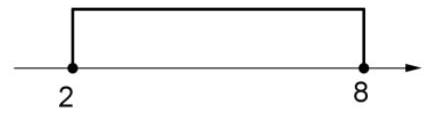
\includegraphics[max width=\textwidth, center]{2024_11_21_b31e6de468170710de69g-02(1)}\\
B.\\
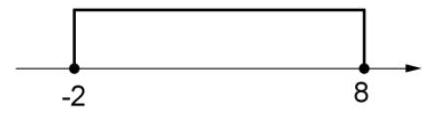
\includegraphics[max width=\textwidth, center]{2024_11_21_b31e6de468170710de69g-02}\\
C.\\
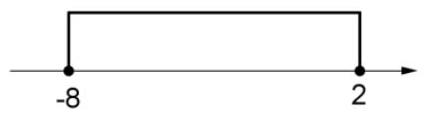
\includegraphics[max width=\textwidth, center]{2024_11_21_b31e6de468170710de69g-02(3)}\\
D.\\
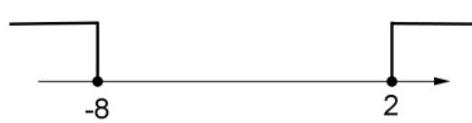
\includegraphics[max width=\textwidth, center]{2024_11_21_b31e6de468170710de69g-02(2)}

\section*{Zadanie 4. (1 pkt)}
Wielomian \(\quad w(x)=(2 x+3)^{3}-(x-5)(x+5) \quad\) przedstawiony \(\quad \mathrm{w}\) postaci sumy algebraicznej przyjmuje postać:\\
A. \(w(x)=8 x^{3}-x^{2}+2\)\\
B. \(w(x)=8 x^{3}-x^{2}+52\)\\
C. \(w(x)=8 x^{3}+35 x^{2}+54 x+52\)\\
D. \(w(x)=8 x^{3}+35 x^{2}+54 x+2\)

Zadanie 5. (1 pkt)\\
Punkt O jest środkiem okręgu. Kąt wpisany \(\alpha\) przedstawiony na rysunku ma miarę:\\
A. \(70^{\circ}\)\\
B. \(110^{\circ}\)\\
C. \(140^{\circ}\)\\
D. \(210^{\circ}\)

Zadanie 6. (1 pkt)\\
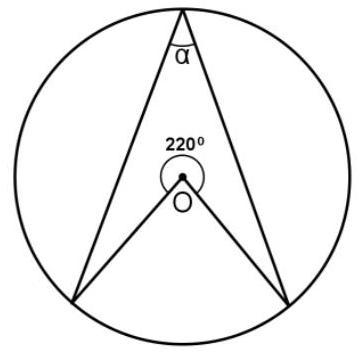
\includegraphics[max width=\textwidth, center]{2024_11_21_b31e6de468170710de69g-02(4)}

Jeżeli \(\operatorname{tg} \alpha=5\), wtedy wartość wyrażenia \(\frac{5 \cos \alpha-4 \sin \alpha}{3 \sin \alpha-4 \cos \alpha}\) jest równa:\\
A. \(-\frac{15}{11}\)\\
B. -1\\
C. \(\frac{15}{11}\)\\
D. \(\frac{21}{11}\)

\section*{BRUDNOPIS}
\begin{center}
\begin{tabular}{|c|c|c|c|c|c|c|c|c|c|c|c|c|c|c|c|c|c|c|c|c|c|c|c|}
\hline
 &  &  &  &  &  &  &  &  &  &  &  &  &  &  &  &  &  &  &  &  &  &  &  \\
\hline
 &  &  &  &  &  &  &  &  &  &  &  &  &  &  &  &  &  &  &  &  &  &  &  \\
\hline
 &  &  &  &  &  &  &  &  &  &  &  &  &  &  &  &  &  &  &  &  &  &  &  \\
\hline
 &  &  &  &  &  &  &  &  &  &  &  &  &  &  &  &  &  &  &  &  &  &  &  \\
\hline
 &  &  &  &  &  &  &  &  &  &  &  &  &  &  &  &  &  &  &  &  &  &  &  \\
\hline
 &  &  &  &  &  &  &  &  &  &  &  &  &  &  &  &  &  &  &  &  &  &  &  \\
\hline
 &  &  &  &  &  &  &  &  &  &  &  &  &  &  &  &  &  &  &  &  &  &  &  \\
\hline
 &  &  &  &  &  &  &  &  &  &  &  &  &  &  &  &  &  &  &  &  &  &  &  \\
\hline
 &  &  &  &  &  &  &  &  &  &  &  &  &  &  &  &  &  &  &  &  &  &  &  \\
\hline
 &  &  &  &  &  &  &  &  &  &  &  &  &  &  &  &  &  &  &  &  &  &  &  \\
\hline
 &  &  &  &  &  &  &  &  &  &  &  &  &  &  &  &  &  &  &  &  &  &  &  \\
\hline
 &  &  &  &  &  &  &  &  &  &  &  &  &  &  &  &  &  &  &  &  &  &  &  \\
\hline
 &  &  &  &  &  &  &  &  &  &  &  &  &  &  &  &  &  &  &  &  &  &  &  \\
\hline
 &  &  &  &  &  &  &  &  &  &  &  &  &  &  &  &  &  &  &  &  &  &  &  \\
\hline
 &  &  &  &  &  &  &  &  &  &  &  &  &  &  &  &  &  &  &  &  &  &  &  \\
\hline
 &  &  &  &  &  &  &  &  &  &  &  &  &  &  &  &  &  &  &  &  &  &  &  \\
\hline
 &  &  &  &  &  &  &  &  &  &  &  &  &  &  &  &  &  &  &  &  &  &  &  \\
\hline
 &  &  &  &  &  &  &  &  &  &  &  &  &  &  &  &  &  &  &  &  &  &  &  \\
\hline
 &  &  &  &  &  &  &  &  &  &  &  &  &  &  &  &  &  &  &  &  &  &  &  \\
\hline
 &  &  &  &  &  &  &  &  &  &  &  &  &  &  &  &  &  &  &  &  &  &  &  \\
\hline
 &  &  &  &  &  &  &  &  &  &  &  &  &  &  &  &  &  &  &  &  &  &  &  \\
\hline
 &  &  &  &  &  &  &  &  &  &  &  &  &  &  &  &  &  &  &  &  &  &  &  \\
\hline
 &  &  &  &  &  &  &  &  &  &  &  &  &  &  &  &  &  &  &  &  &  &  &  \\
\hline
 &  &  &  &  &  &  &  &  &  &  &  &  &  &  &  &  &  &  &  &  &  &  &  \\
\hline
 &  &  &  &  &  &  &  &  &  &  &  &  &  &  &  &  &  &  &  &  &  &  &  \\
\hline
 &  &  &  &  &  &  &  &  &  &  &  &  &  &  &  &  &  &  &  &  &  &  &  \\
\hline
 &  &  &  &  &  &  &  &  &  &  &  &  &  &  &  &  &  &  &  &  &  &  &  \\
\hline
 &  &  &  &  &  &  &  &  &  &  &  &  &  &  &  &  &  &  &  &  &  &  &  \\
\hline
 &  &  &  &  &  &  &  &  &  &  &  &  &  &  &  &  &  &  &  &  &  &  &  \\
\hline
 &  &  &  &  &  &  &  &  &  &  &  &  &  &  &  &  &  &  &  &  &  &  &  \\
\hline
 &  &  &  &  &  &  &  &  &  &  &  &  &  &  &  &  &  &  &  &  &  &  &  \\
\hline
 &  &  &  &  &  &  &  &  &  &  &  &  &  &  &  &  &  &  &  &  &  &  &  \\
\hline
 &  &  &  &  &  &  &  &  &  &  &  &  &  &  &  &  &  &  &  &  &  &  &  \\
\hline
 &  &  &  &  &  &  &  &  &  &  &  &  &  &  &  &  &  &  &  &  &  &  &  \\
\hline
 &  &  &  &  &  &  &  &  &  &  &  &  &  &  &  &  &  &  &  &  &  &  &  \\
\hline
 &  &  &  &  &  &  &  &  &  &  &  &  &  &  &  &  &  &  &  &  &  &  &  \\
\hline
 &  &  &  &  &  &  &  &  &  &  &  &  &  &  &  &  &  &  &  &  &  &  &  \\
\hline
 &  &  &  &  &  &  &  &  &  &  &  &  &  &  &  &  &  &  &  &  &  &  &  \\
\hline
 &  &  &  &  &  &  &  &  &  &  &  &  &  &  &  &  &  &  &  &  &  &  &  \\
\hline
 &  &  &  &  &  &  &  &  &  &  &  &  &  &  &  &  &  &  &  &  &  &  &  \\
\hline
 &  &  &  &  &  &  &  &  &  &  &  &  &  &  &  &  &  &  &  &  &  &  &  \\
\hline
 &  &  &  &  &  &  &  &  &  &  &  &  &  &  &  &  &  &  &  &  &  &  &  \\
\hline
 &  &  &  &  &  &  &  &  &  &  &  &  &  &  &  &  &  &  &  &  &  &  &  \\
\hline
 &  &  &  &  &  &  &  &  &  &  &  &  &  &  &  &  &  &  &  &  &  &  &  \\
\hline
\end{tabular}
\end{center}

Zadanie 7. (1 pkt)\\
Zdanie „różnica kwadratów dwóch kolejnych liczb naturalnych nieparzystych jest niemniejsza niż 5" przedstawiono w postaci nierówności:\\
A. \((n+3)^{2}-(n+1)^{2} \geq 5\)\\
B. \((2 n+3)^{2}-(2 n+1)^{2} \geq 5\)\\
C. \((2 n+3)^{2}-(2 n+1)^{2}>5\)\\
D. \([(2 n+3)-(2 n+1)]^{2} \geq 5\)

Zadanie 8. (1 pkt)\\
Na rysunku przedstawiony jest wykres pewnej funkcji \(y=f(x)\). Przyjmuje ona wartości niedodatnie dla argumentów:\\
A. \(x \in(-4,1) \cup(3,6)\)\\
B. \(x \in\langle-4,1\rangle \cup\langle 3,6\rangle\)\\
C. \(x \in\langle(-6,-4) \cup(1,3) \cup(6,7\rangle\)\\
D. \(x \in(-4,6)\)\\
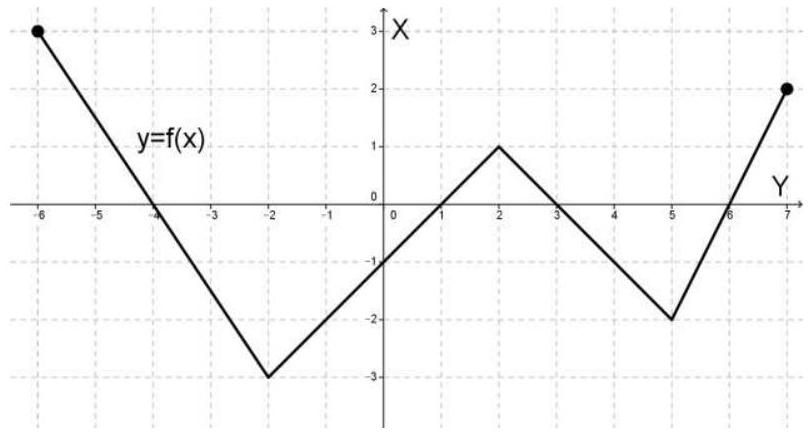
\includegraphics[max width=\textwidth, center]{2024_11_21_b31e6de468170710de69g-04}

\section*{Zadanie 9. (1 pkt)}
Wyrażenie \(\frac{\log _{2} 32}{\log _{2} 16}\) ma wartość równą:\\
A. \(\log _{2} 16\)\\
B. \(\log _{2} 2\)\\
C. \(\frac{5}{4}\)\\
D. 2

Zadanie 10. (1 pkt)\\
W ciągu arytmetycznym wyraz \(a_{2}=-2, a_{7}=-7\). Wtedy:\\
A. \(a_{2014}=-2015\)\\
B. \(a_{2014}=-2014\)\\
C. \(a_{2014}=2011\)\\
D. \(a_{2014}=2014\)

Zadanie 11. (1 pkt)\\
Rozwiązaniem nierówności \(7 x \leq x^{2}\) jest zbiór:\\
A. \(x \in(-\infty, 0) \cup(7,+\infty)\)\\
B. \(x \in\langle 0,7\rangle\)\\
C. \(x \in\langle 7,+\infty)\)\\
D. \(x \in(-\infty, 0\rangle \cup\langle 7,+\infty)\)

Zadanie 12. (1 pkt)\\
Dla \(x \in R \backslash\{-3,-2,3\}\) wyrażenie \(\frac{1}{(x-3)(x+2)}-\frac{2}{x^{2}-9}\) jest równe:\\
A. \(\frac{-x-1}{\left(x^{2}-9\right)(x+2)}\)\\
B. \(\frac{-x+7}{\left(x^{2}-9\right)(x+2)}\)\\
C. \(\frac{x+1}{\left(x^{2}-9\right)(x+2)}\)\\
D. \(\frac{-2 x-3}{\left(x^{2}-9\right)(x+2)}\)

Zadanie 13. (1 pkt)\\
Wartość wyrażenia \(\sin 43^{\circ} \cos 47^{\circ}+\cos 43^{\circ} \sin 47^{\circ}\) jest równa:\\
A. -1\\
B. 0\\
C. 1\\
D. 2

\section*{BRUDNOPIS}
\begin{center}

\includegraphics[max width=\textwidth]{2024_11_21_b31e6de468170710de69g-05}
\end{center}

Zadanie 14. (1 pkt)\\
Średnia danych przestawionych na wykresie słupkowym jest równa:\\
A. 8,25\\
B. 4

C 3,3\\
D. 0,625

Zadanie 15. (1 pkt)\\
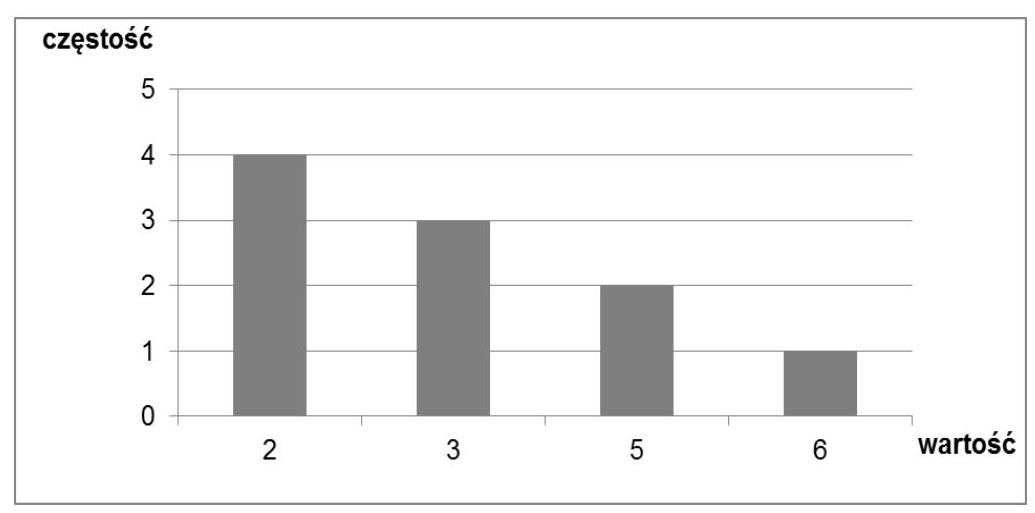
\includegraphics[max width=\textwidth, center]{2024_11_21_b31e6de468170710de69g-06}

Liczba \(-\frac{3}{2} \log 4+\frac{5}{3} \log 8\) jest równa:\\
A. \(2 \log 2\)\\
B. \(\log 24\)\\
C. 2\\
D. \(8 \log 2\)

Zadanie 16. (1 pkt)\\
Wielokąt o polu \(180 \mathrm{~cm}^{2}\) przekształcono przez podobieństwo o skali \(k\) tak, że jego pole zmniejszyło się o \(100 \mathrm{~cm}^{2}\). Skala \(k\) podobieństwa jest równa:\\
A. \(k=\frac{4}{9}\)\\
B. \(k=\frac{2}{3}\)\\
C. \(k=\frac{10}{18}\)\\
D. \(k=\frac{16}{81}\)

Zadanie 17. (1pkt)\\
Równanie prostej równoległej do prostej \(y=\frac{1}{2} x\) przechodzącej przez punkt \(A=(0,-2)\) ma postać:\\
A. \(y=\frac{1}{2} x-2\)\\
B. \(y=-2 x-2\)\\
C. \(y=-\frac{1}{2} x-2\)\\
D. \(y=2 x-2\)

Zadanie 18. (1 pkt)\\
Na rysunku obok przedstawiono wykres funkcji \(y=f(x)\).\\
Wzór opisujący funkcję \(y=f(x)\) ma postać:\\
A. \(f(x)=-3 x-2\)\\
B. \(f(x)=-2 x-2\)\\
C. \(f(x)=2 x-2\)\\
D. \(f(x)=3 x-2\)

Zadanie 19. (1 pkt)\\
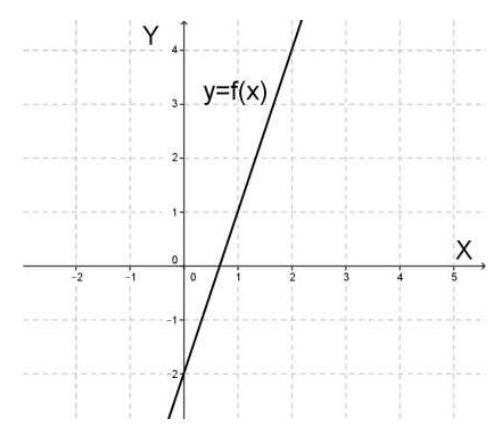
\includegraphics[max width=\textwidth, center]{2024_11_21_b31e6de468170710de69g-06(1)}

Ciągiem geometrycznym jest ciąg \(\left(a_{n}\right)\) o wyrazie ogólnym:\\
A. \(a_{n}=\mathrm{n}^{2}-3\)\\
B. \(a_{n}=3 \mathrm{n}+2\)\\
C. \(a_{n}=5 \cdot 3^{\mathrm{n}}\)\\
D. \(a_{n}=\frac{4}{n}\)

Zadanie 20. (1 pkt)\\
Przekątna sześcianu jest o 3 dłuższa od długości jego krawędzi. Długość krawędzi sześcianu jest równa\\
A. \(\frac{3 \sqrt{3}-3}{2}\)\\
B. \(\frac{3 \sqrt{3}+3}{2}\)\\
C. \(3 \sqrt{3}+3\)\\
D. \(\sqrt{3}+3\)

\section*{BRUDNOPIS}
Materiały pobrane z serwisu \href{http://www.zadania.info}{www.zadania.info}\\

\includegraphics[max width=\textwidth, center]{2024_11_21_b31e6de468170710de69g-07}

Zadanie 21. (1 pkt)\\
Wielomian \(W(x)=x^{4}-3 x^{3}+4 x^{2}-12 x\) po rozłożeniu na czynniki ma postać:\\
A. \(W(x)=(x-3)^{2}\left(x^{2}+4\right)\)\\
B. \(W(x)=x\left(x^{2}+3\right)(x-4)\)\\
C. \(W(x)=x(x+2)(x-2)(x-3)\)\\
D. \(W(x)=x\left(x^{2}+4\right)(x-3)\)

Zadanie 22. (1 pkt)\\
Na rysunku przedstawiony jest wykres funkcji \(y=f(x)\) oraz \(y=g(x)\). Wówczas:\\
A. \(g(x)=f(x+3)+4\)\\
B. \(g(x)=f(x-3)+4\)\\
C. \(g(x)=f(x+4)+3\)\\
D. \(g(x)=f(x-4)+3\)

Zadanie 23. (1 pkt)\\
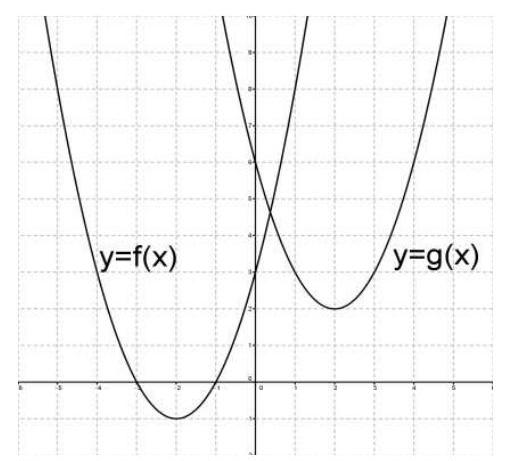
\includegraphics[max width=\textwidth, center]{2024_11_21_b31e6de468170710de69g-08(1)}

Ze zbioru liczb \(\{1,2,3,4,5,6,7\}\) losujemy kolejno dwa razy po jednej cyfrze bez zwracania.\\
Zapisując wylosowane cyfry w kolejności losowania, otrzymujemy liczbę dwucyfrową.\\
Prawdopodobieństwo otrzymania liczby większej od 32 jest równe:\\
A. \(\frac{28}{49}\)\\
B. \(\frac{29}{49}\)\\
C. \(\frac{28}{42}\)\\
D. \(\frac{29}{42}\)

Zadanie 24. (1 pkt)\\
Jeżeli \(S=(-2,3)\) jest środkiem odcinka o końcach \(A=(0, a)\) i \(B=(b,-1)\), to:\\
A. \(a+b=3\)\\
B. \(a+b=2\)\\
C. \(a+b=1\)\\
D. \(a+b=0\)

Zadanie 25. (1 pkt)\\
Wykres funkcji \(f(x)=-2(x+3)^{2}+1\) przedstawiony jest na rysunku:\\
A.\\
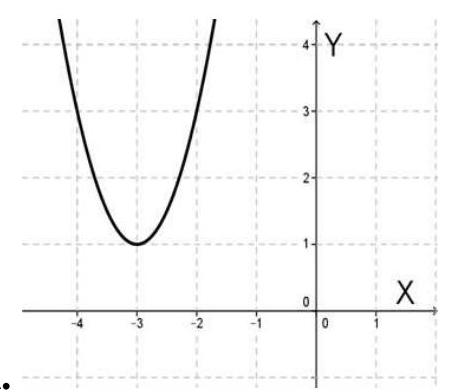
\includegraphics[max width=\textwidth, center]{2024_11_21_b31e6de468170710de69g-08}\\
B.\\
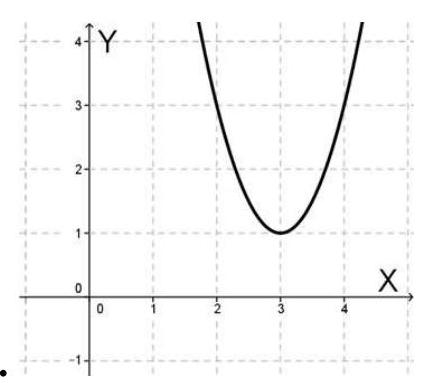
\includegraphics[max width=\textwidth, center]{2024_11_21_b31e6de468170710de69g-08(4)}\\
C.\\
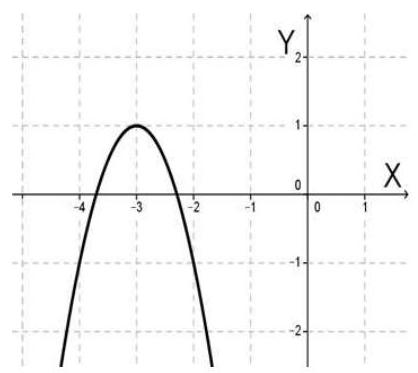
\includegraphics[max width=\textwidth, center]{2024_11_21_b31e6de468170710de69g-08(3)}\\
D.\\
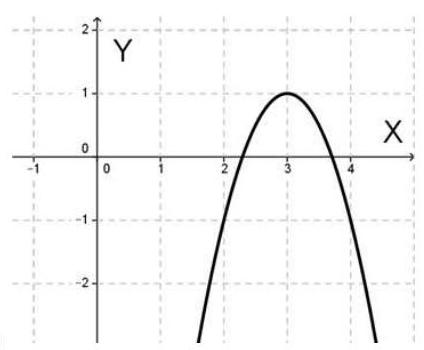
\includegraphics[max width=\textwidth, center]{2024_11_21_b31e6de468170710de69g-08(2)}

\section*{BRUDNOPIS}
Materiaty pobrane z serwisu \href{http://www.zadania.info}{www.zadania.info}\\

\includegraphics[max width=\textwidth, center]{2024_11_21_b31e6de468170710de69g-09}

\section*{ZADANIA OTWARTE}
Rozwiazania zadań o numerach od 26. do 34. należy zapisać w wyznaczonych miejscach pod treścia zadania.\\
Zadanie 26. (2 pkt)\\
Rozwiąż równanie: \(\frac{3 x-6}{x^{2}-4}=2\).\\

\includegraphics[max width=\textwidth, center]{2024_11_21_b31e6de468170710de69g-10}

Odpowiedź:\\
Zadanie 27. (2 pkt)\\
Wykaż, że dwusieczne dwóch sąsiednich kątów równoległoboku są prostopadłe.\\
\(\qquad\)

Zadanie 28. (2 pkt)\\
Wyznacz najmniejszą i największą wartość funkcji kwadratowej \(y=x^{2}-4 x+1\) w przedziale \(\langle 3,5\rangle\).\\

\includegraphics[max width=\textwidth, center]{2024_11_21_b31e6de468170710de69g-11}

Odpowiedź:

Zadanie 29. (2 pkt)\\
Ze zbioru liczb trzycyfrowych mniejszych od 500 wybieramy losowo jedną liczbę. Jakie jest prawdopodobieństwo, że będzie to liczba podzielna przez 3 lub przez 5?\\

\includegraphics[max width=\textwidth, center]{2024_11_21_b31e6de468170710de69g-12}

Odpowiedź:

Zadanie 30. (2 pkt)\\
Wykaż, że jeżeli \(x+y=5\), to \(x^{2}+y^{2} \geq \frac{25}{2}\).\\

\includegraphics[max width=\textwidth, center]{2024_11_21_b31e6de468170710de69g-13}

\section*{Zadanie 31. (2 pkt)}
Przekątne \(A C \quad\) i \(B D\) rombu \(A B C D\) przecinają się w punkcie \(S=(6,-4)\). Wyznacz równanie prostej zawierającej przekątną \(A C\) wiedząc, że prosta zawierająca przekątną \(B D\) ma równanie \(3 x-4 y-34=0\).\\

\includegraphics[max width=\textwidth, center]{2024_11_21_b31e6de468170710de69g-14}

Odpowiedź:

Zadanie 32. (4 pkt)\\
Objętość graniastosłupa prawidłowego czworokątnego jest równa \(224 \mathrm{~cm}^{3}\), promień okręgu opisanego na podstawie ma długość 4 cm . Wyznacz miarę kąta między przekątnymi sąsiednich ścian bocznych wychodzącymi z tego samego wierzchołka graniastosłupa.\\

\includegraphics[max width=\textwidth, center]{2024_11_21_b31e6de468170710de69g-15}

Odpowiedź:

\section*{Zadanie 33. (4 pkt)}
Samochód przejechał \(\frac{1}{4}\) trasy ze średnią prędkością \(80 \mathrm{~km} / \mathrm{h}\). Na całej trasie średnia prędkość samochodu była równa \(64 \mathrm{~km} / \mathrm{h}\). Oblicz z jaką średnią prędkością samochód przejechał pozostałą część trasy.\\

\includegraphics[max width=\textwidth, center]{2024_11_21_b31e6de468170710de69g-16}\\
\(\qquad\)\\
Odpowiedź:

Zadanie 34. (5 pkt)\\
W trójkącie prostokątnym \(A B C\) o przeciwprostokątnej \(A B\) dane są wierzchołki \(A=(-1,-4)\) i \(C=(5,2)\). Punkt \(B\) leży na prostej o równaniu \(y=2 x-2\). Wyznacz równanie okręgu opisanego na tym trójkącie.\\

\includegraphics[max width=\textwidth, center]{2024_11_21_b31e6de468170710de69g-18}\\
\(\qquad\)\\
Odpowiedź:

\section*{PESEL}
WYPEENIA ZDAJĄCY

\begin{center}
\begin{tabular}{|c|c|c|c|c|}
\hline
\multirow{2}{*}{\begin{tabular}{l}
Nr \\
zad. \\
\end{tabular}} & \multicolumn{4}{|c|}{Odpowiedzi} \\
\hline
 & A & B & C & D \\
\hline
1 & ㅁ & ㅁ & ㅁ & ■ \\
\hline
2 & ㅁ & ㅁ & ㅁ & ㅁ \\
\hline
3 & ㅁ & ㅁ & ㅁ & - \\
\hline
4 & ㅁ & ㅁ & ㅁ & ㅁ \\
\hline
5 & ㅁ & ㅁ & ㅁ & ㅁ \\
\hline
6 & ㅁ & ㅁ & ㅁ & ㅁ \\
\hline
7 & ㅁ & ㅁ & ㅁ & ㅁ \\
\hline
8 & ㅁ & ㅁ & ㅁ & ㅁ \\
\hline
9 & ㅁ & ㅁ & ㅁ & ㅁ \\
\hline
10 & ㅁ & ㅁ & ㅁ & ㅁ \\
\hline
11 & ㅁ & ㅁ & ㅁ & ㅁ \\
\hline
12 & ㅁ & ㅁ & ㅁ & ㅁ \\
\hline
13 & ㅁ & ㅁ & ㅁ & ㅁ \\
\hline
14 & ㅁ & ㅁ & ㅁ & ㅁ \\
\hline
15 & ㅁ & ㅁ & - & - \\
\hline
16 & ㅁ & ㅁ & ㅁ & ㅁ \\
\hline
17 & ㅁ & ㅁ & ㅁ & ㅁ \\
\hline
18 & ㅁ & ㅁ & ㅁ & \(\square\) \\
\hline
19 & ㅁ & ㅁ & ㅁ & ㅁ \\
\hline
20 & ㅁ & ㅁ & - & ㅁ \\
\hline
21 & ㅁ & ㅁ & ㅁ & ㅁ \\
\hline
22 & ㅁ & ㅁ & ㅁ & ㅁ \\
\hline
23 & ㅁ & ㅁ & ㅁ & ㅁ \\
\hline
24 & ㅁ & ㅁ & ㅁ & ㅁ \\
\hline
25 & ㅁ & ㅁ & ㅁ & - \\
\hline
\end{tabular}
\end{center}

WYPELNIA EGZAMINATOR

\begin{center}
\begin{tabular}{|c|c|c|c|c|c|c|}
\hline
\multirow{2}{*}{\begin{tabular}{c}
Nr \\
zad. \\
\end{tabular}} & \multicolumn{6}{|c|}{Punkty} \\
\hline
 & \(\mathbf{0}\) & \(\mathbf{1}\) & \(\mathbf{2}\) & \(\mathbf{3}\) & \(\mathbf{4}\) & \(\mathbf{5}\) \\
\hline
\(\mathbf{2 6}\) & \(\square\) & \(\square\) & \(\square\) &  &  &  \\
\hline
\(\mathbf{2 7}\) & \(\square\) & \(\square\) & \(\square\) &  &  &  \\
\hline
\(\mathbf{2 8}\) & \(\square\) & \(\square\) & \(\square\) &  &  &  \\
\hline
\(\mathbf{2 9}\) & \(\square\) & \(\square\) & \(\square\) &  &  &  \\
\hline
\(\mathbf{3 0}\) & \(\square\) & \(\square\) & \(\square\) &  &  &  \\
\hline
\(\mathbf{3 1}\) & \(\square\) & \(\square\) & \(\square\) &  &  &  \\
\hline
\(\mathbf{3 2}\) & \(\square\) & \(\square\) & \(\square\) & \(\square\) & \(\square\) &  \\
\hline
\(\mathbf{3 3}\) & \(\square\) & \(\square\) & \(\square\) & \(\square\) & \(\square\) &  \\
\hline
\(\mathbf{3 4}\) & \(\square\) & \(\square\) & \(\square\) & \(\square\) & \(\square\) & \(\square\) \\
\hline
\end{tabular}
\end{center}

SUMA PUNKTÓW\\

\includegraphics[max width=\textwidth, center]{2024_11_21_b31e6de468170710de69g-20}


\end{document}